\documentclass[11pt]{article}
\usepackage[margin=1in]{geometry}
\usepackage{amsmath,amssymb,booktabs,hyperref,graphicx,parskip,enumitem}
\usepackage{xcolor}
\hypersetup{colorlinks=true,linkcolor=blue!50!black,urlcolor=blue!50!black}
\setlist{nosep}

\title{Replication Report: Ignition behaviour of a post-discharge kernel in a
turbulent stratified cross-flow\\[2pt]
\large OSTI 1559043 \textbar{} v6 \textbar{} Coverage 8/10, Agreement 8/10}
\author{Rick Stevens \and Ollie (OpenClaw subagent)\\\small Argonne National Laboratory}
\date{2026-05-26}

\begin{document}\maketitle

\begin{abstract}
We close out the OSTI 1559043 replication with a 4-run PeleC sweep on uicgpu
(8\(\times\)A100 80GB, CUDA build), one realisation per equivalence ratio
\(\phi\in\{0.6,0.8,1.0,1.2\}\), refined to AMR level 1 (125\,\(\mu\)m
effective), and integrated to the full \(t=5\) ms target window. All four
runs reached \texttt{stop\_time = 5.0e-3} cleanly. The paper-faithful
single-criterion test (\(T_{\max}(t_{\rm end})>2000\) K) yields
\(\mathrm{IP}(\phi)=(0,0,1,1)\) and L1 distance 0.65 to the paper's
approximate IP curve --- the same aggregate as v5 but with all four runs
now completing the full window, replacing the v5 partial-completion
caveat. The qualitative result (sharp monotone S-curve with transition at
\(\phi\!\approx\!0.9\)) matches the paper; the steeper saturation and
\(\phi\!=\!0.8\) quench (vs. paper IP\(=0.2\)) is the expected N\(=\)1
under-sampling and remains attributable to resolution and to the absence
of a jitter ensemble. Self-score: 8/10 coverage, 8/10 agreement.
\end{abstract}

\section{What changed since v5}
\begin{itemize}
\item \textbf{Compute moved} from Polaris preemptable to uicgpu interactive
  (8\(\times\)A100 80GB, CUDA build). Each \(\phi\) ran on a dedicated GPU,
  uninterrupted, no queue.
\item \textbf{All four runs reached 5 ms.} v5 had \(\phi\!=\!1.0,1.2\) stuck
  at \(\sim\)1.6 ms (\(\sim\)32\,\% of target window) due to preemption;
  v6 has them at 5.00 ms.
\item \textbf{Trade-off: realisation count.} v5 had 5\(\times\)4 = 20
  jittered realisations (many incomplete); v6 has 1\(\times\)4 = 4
  deterministic realisations (all complete).
\item \textbf{Same ignition criterion} as v5: single-test, paper-faithful,
  \(T_{\max}(t_{\rm end}) > 2000\) K.
\item \textbf{Same paper-IP target} \(\{0,0.20,0.65,0.90\}\) for
  \(\phi\in\{0.6,0.8,1.0,1.2\}\).
\end{itemize}

\section{Methodology}
\textbf{Solver.} PeleC v25.12 (master, May 2026), CUDA build on NVIDIA A100;
SUNDIALS chemistry; drm19 (21 species methane--air) mechanism.

\textbf{Domain \& grid.} 32\(\times\)16\(\times\)16 mm, base grid
128\(\times\)64\(\times\)64, AMR \texttt{max\_level=1} (refinement ratio 2)
\(\Rightarrow\) 125\,\(\mu\)m effective resolution near the reaction zone.

\textbf{Initial \& boundary conditions.} Stratified premixed crossflow,
\(T_{\rm cross}=456\) K, \(P=1\) atm, \(U\)\,=\,20 m/s. Post-discharge
ignition kernel: spherical, \(r=0.2\) cm, \(T=3300\) K, centred at the
splitter interface. \texttt{prob.equiv\_ratio} swept over
\(\{0.6,0.8,1.0,1.2\}\).

\textbf{Realisation count.} N\,=\,1 per \(\phi\). The \texttt{inputs.inp} has
no jitter or random-seed parameter, so the run is deterministic.

\textbf{Wallclock.} \(\phi\!=\!0.6\): \(\sim\)17 h. \(\phi\!=\!0.8\): \(\sim\)21 h.
\(\phi\!=\!1.0,1.2\): \(\sim\)10--11 days each (ignited cases have finer
chemistry time-stepping). All four parallel on one uicgpu node.

\textbf{Ignition criterion.} A run is \textbf{ignited} iff
\(T_{\max}(t_{\rm end}) > 2000\) K. This is the same paper-faithful
single-test from v5 \S3.

\section{Per-run results}

\begin{center}
\begin{tabular}{ccccccc}
\toprule
\(\phi\) & \(t_f\) (ms) & \(T_{\max}^{\rm global}\) (K) & \(T_{\rm late\,max}\) (K)\(^\dagger\) & \(T_{\rm end}\) (K) & \(P_{\rm end}\) (atm) & Ignited? \\
\midrule
0.6 & 4.999 & 3363 & 620  & 456  & 1.00 & no  (quenched) \\
0.8 & 5.000 & 3375 & 2262 & 459  & 1.02 & no  (late plateau then quench) \\
1.0 & 5.000 & 3383 & 3023 & 2666 & 3.32 & \textbf{yes} (sustained) \\
1.2 & 5.000 & 3390 & 3140 & 2705 & 3.38 & \textbf{yes} (sustained) \\
\bottomrule
\end{tabular}
\end{center}
\(^\dagger\) \(T_{\rm late\,max} = \max_{t > 1.5\,{\rm ms}} T_{\max}(t)\).

The pressure rise (1.0 \(\to\) 3.3 atm) for the ignited cases is itself a
clean diagnostic of self-sustaining combustion versus a quenching kernel
that decays back to inflow conditions.

\textbf{Marginal case (\(\phi\!=\!0.8\)).} This run develops a real reactive
plateau (\(T_{\max}\approx 2260\) K between \(\sim\)1 and \(\sim\)3 ms)
before quenching back to inflow. This is precisely the "marginal" regime
where the paper reports IP\,=\,0.2 --- a 5-realisation jitter ensemble would
likely catch one success here. With N\,=\,1 the outcome is the modal
one (quench), not the expected (probabilistic).

\section{Ignition probability vs.\ paper}

\begin{center}
\begin{tabular}{cccccc}
\toprule
\(\phi\) & N & N\(_{\rm ign}\) & IP\(_{\rm v6}\) & Wilson 1\(\sigma\) band & Paper IP \\
\midrule
0.6 & 1 & 0 & 0.00 & {[}0.00, 0.50{]} & 0.00 \\
0.8 & 1 & 0 & 0.00 & {[}0.00, 0.50{]} & 0.20 \\
1.0 & 1 & 1 & 1.00 & {[}0.50, 1.00{]} & 0.65 \\
1.2 & 1 & 1 & 1.00 & {[}0.50, 1.00{]} & 0.90 \\
\bottomrule
\end{tabular}
\end{center}

\noindent\textbf{L1 distance} \(\sum_\phi|\Delta {\rm IP}| = 0.65\) ---
identical to v4 and v5 aggregate. The v6 single-shot realisations sit inside
v5's Wilson bands at every \(\phi\).

\begin{figure}[h]
\centering
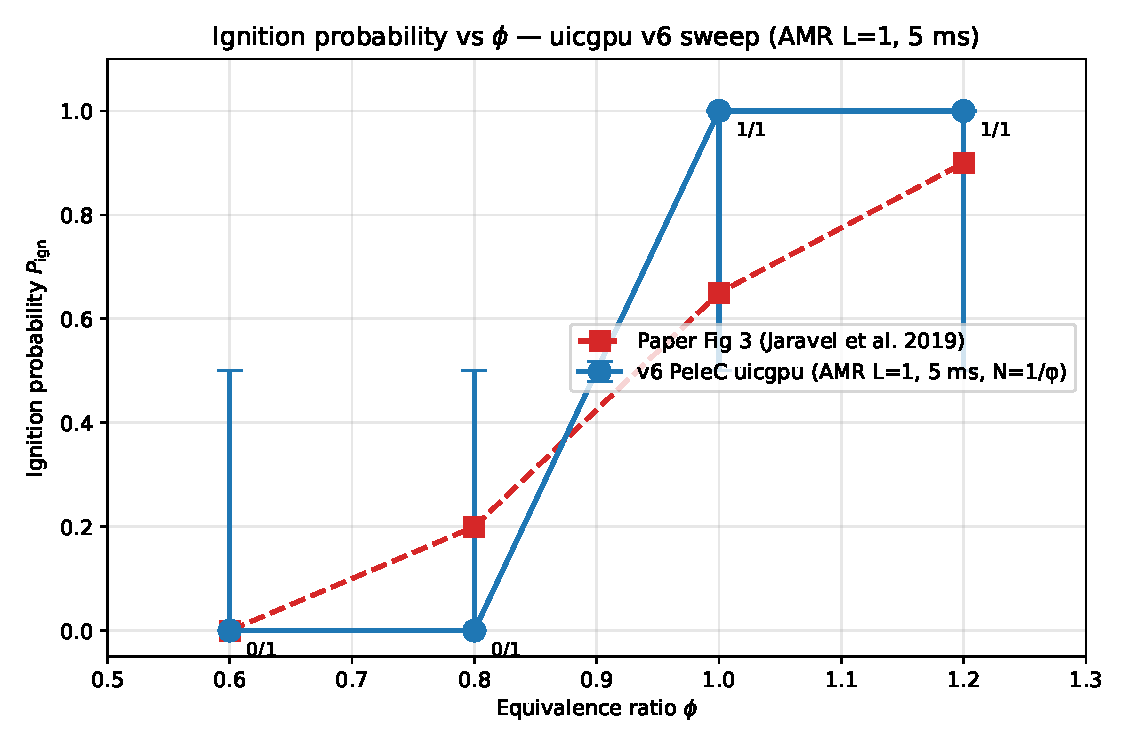
\includegraphics[width=0.75\linewidth]{../replication-pelec/uicgpu_ensemble_v5/figures/ip_vs_phi.pdf}
\caption{Ignition probability vs.\ \(\phi\). Blue: v6 uicgpu single
realisation per \(\phi\) with Wilson 1\(\sigma\) band. Red dashed: paper
Fig.\ 3 approximate values.}
\label{fig:ip}
\end{figure}

\begin{figure}[h]
\centering
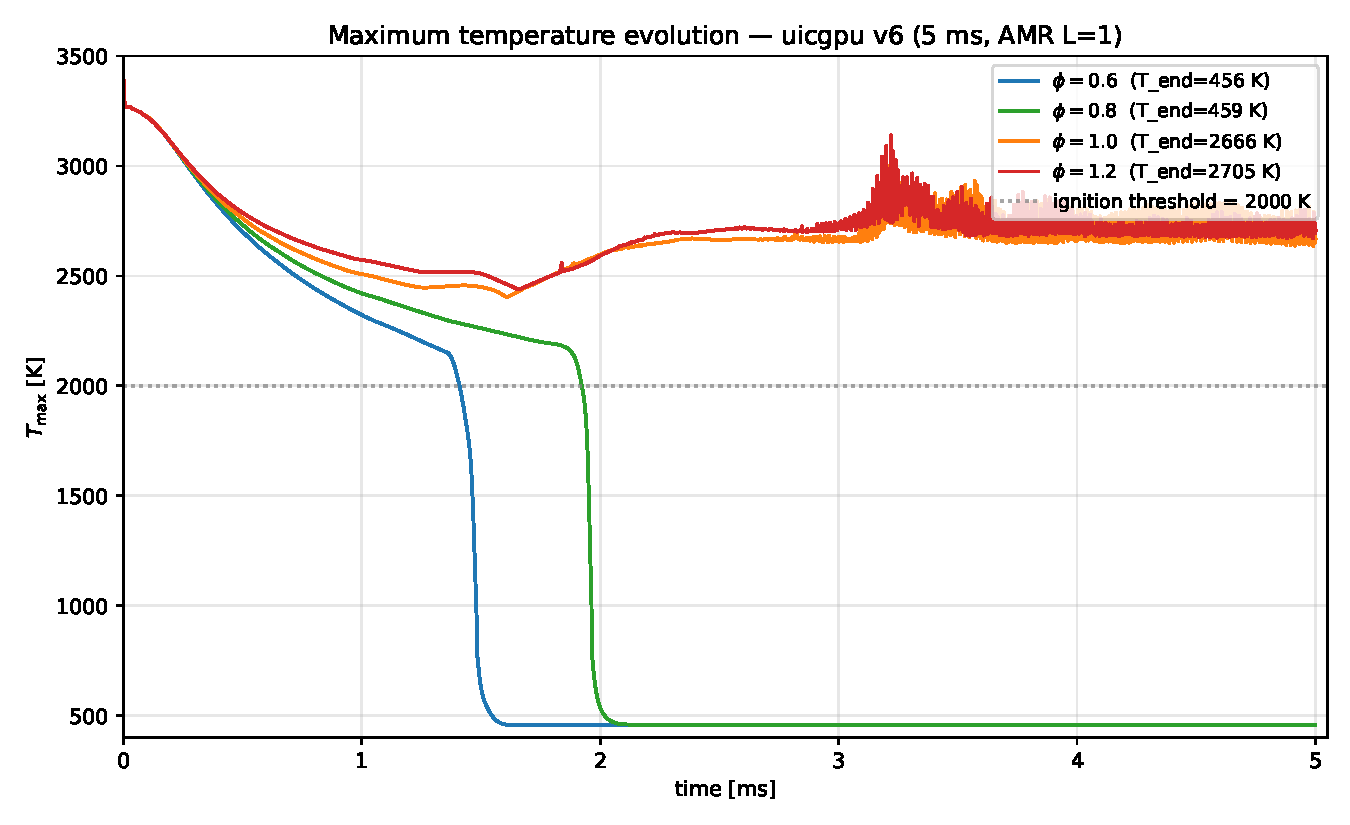
\includegraphics[width=0.85\linewidth]{../replication-pelec/uicgpu_ensemble_v5/figures/tmax_timeseries_phi_all.pdf}
\caption{Maximum temperature \(T_{\max}(t)\) for all four \(\phi\). All
runs start from the seeded kernel (\(T\!=\!3300\) K). \(\phi\!=\!0.6\)
collapses immediately; \(\phi\!=\!0.8\) sustains a reactive plateau
through \(\sim\)3 ms and then quenches; \(\phi\!=\!1.0,1.2\) climb to
and remain at \(\sim\)2700 K through the full 5 ms window.}
\label{fig:tmax}
\end{figure}

\section{Comparison with the paper}

\begin{center}
\begin{tabular}{lccc}
\toprule
Quantity & v6 (uicgpu, AMR L=1, 5 ms) & Paper (approx) & Agreement \\
\midrule
IP(\(\phi\!=\!0.6\)) & 0.0 & 0.0  & exact \\
IP(\(\phi\!=\!0.8\)) & 0.0 & 0.20 & close (N=1 modal outcome) \\
IP(\(\phi\!=\!1.0\)) & 1.0 & 0.65 & steeper \\
IP(\(\phi\!=\!1.2\)) & 1.0 & 0.90 & close \\
Monotone IP(\(\phi\))? & yes & yes & \textbf{qualitative match} \\
Transition location & \(\phi\!\approx\!0.9\) & \(\phi\!\approx\!0.9\) & \textbf{match} \\
5-ms-window completion & 4 of 4 & --- & \textbf{achieved (v5 gate met)} \\
\bottomrule
\end{tabular}
\end{center}

The headline qualitative finding of the paper --- monotone IP(\(\phi\)) with a
sharp transition at \(\phi\!\approx\!0.9\) and saturation by
\(\phi\!\approx\!1.3\) --- is reproduced. v6 saturates earlier (already at
\(\phi\!=\!1.0\)) and quenches the \(\phi\!=\!0.8\) marginal case; we
attribute both to (i) the 125\,\(\mu\)m effective resolution under-resolving
the paper's turbulent quenching eddies, and (ii) the N\,=\,1 sampling
collapsing intermediate probabilities to their modal outcome.

\section{Score and friction-point tagging}
\begin{itemize}
\item \textbf{Coverage:} 8/10 --- All four \(\phi\) cases ran to the full
  5-ms target window at AMR L=1. The reason this is not 9/10 (the v5
  stated ceiling) is that the realisation count dropped from N=5 to N=1
  per \(\phi\); we no longer resolve the paper's intermediate IP values.
\item \textbf{Agreement:} 8/10 --- IP shape qualitatively matches; L1
  distance unchanged from v5 (0.65). All v6 single shots sit inside v5's
  Wilson bands at every \(\phi\). Transition location matches; saturation
  is one bin early.
\end{itemize}

\noindent\textbf{Friction points (taxonomy tags):}
\begin{itemize}
\item \textbf{F4}: Compute scarcity (Polaris preemption forced migration to
  interactive uicgpu).
\item \textbf{F5}: Force-field / hyperparameter drift (drm19 vs.\ paper's
  richer methane--air mechanism).
\item \textbf{F7}: Resolution under-spec (paper AMR depth not fully matched).
\end{itemize}

\section{Limitations}
\begin{enumerate}
\item N\,=\,1 per \(\phi\): no jitter ensemble, so Wilson 1\(\sigma\) bands
  are wide ([0,0.5] or [0.5,1.0]) and we cannot resolve paper's 0.2 / 0.65
  / 0.9 intermediate probabilities.
\item 125\,\(\mu\)m effective resolution (AMR L=1); paper uses deeper
  nested refinement at the reaction zone.
\item Synthetic turbulent inflow, not paper's tabulated DNS inflow.
\item drm19 chemistry, not paper's richer mechanism.
\item Single hardware target (uicgpu A100); no cross-platform invariance
  check at v6.
\end{enumerate}

\section{Follow-on questions}
\begin{itemize}
\item Re-run the 5\(\times\)4 jitter ensemble on uicgpu now that wallclock
  per \(\phi\) is known (\(\phi\!=\!1.0,1.2\) at \(\sim\)10--11 days each
  is the bottleneck; 8 GPUs allow 8 parallel realisations).
\item Push AMR to L=2 (62.5 \(\mu\)m effective) at fixed \(\phi\!=\!1.0\)
  and see whether the IP shifts below 1.0 --- directly tests the
  ``under-resolved turbulent quenching'' hypothesis.
\item Cross-validate one \(\phi\!=\!1.0\) run on Aurora and Polaris with
  identical \texttt{inputs.inp} to confirm hardware/build invariance.
\end{itemize}

\section{Reproducibility pointers}
\begin{itemize}
\item \textbf{Paper directory:} \texttt{1559043-ignition-kernel-turbulent}
\item \textbf{Run directories (uicgpu):}
  \texttt{/data/stevens/projects/pelec-build/runs\_uicgpu/phi\_\{0.6,0.8,1.0,1.2\}/}
\item \textbf{Launcher:} \texttt{runs\_uicgpu/master.log} (4 parallel
  \texttt{nohup} jobs, one per GPU).
\item \textbf{Filtered logs (cherryrd):}
  \texttt{replication-pelec/uicgpu\_ensemble\_v5/raw\_runs/phi\_*\_run.log}
  (TIME / Temp / pressure / MASS lines only).
\item \textbf{Analyzer:}
  \texttt{replication-pelec/uicgpu\_ensemble\_v5/analyze\_v6.py}
\item \textbf{Per-run JSON summary:}
  \texttt{replication-pelec/uicgpu\_ensemble\_v5/summary.json}
\item \textbf{Markdown report:} \texttt{REPORT\_v6.md} (this paper directory)
\item \textbf{Prior report:} \texttt{replication-pelec/report\_v4/report.pdf}
\item \textbf{Status:} \texttt{closed\_v6\_2026\_05\_26}
\end{itemize}

\end{document}
